\section[BÀI TOÁN THỰC TIỄN VÀ CHỨC NĂNG]{BÀI TOÁN THỰC TIỄN VÀ CHỨC NĂNG HỆ THỐNG}
\label{sec:chuong1}

\subsection{Mô tả bài toán}
\label{subsec:baitoan}

Trong bài toán mô phỏng, một phường có nhiều tổ dân phố, mỗi tổ có cán bộ theo dõi dân cư trong tổ. Cán bộ cần nắm danh sách địa chỉ, các hộ ở mỗi địa chỉ, các thành viên trong hộ và việc họ thường trú hay tạm trú trong từng khoảng thời gian. Các thông tin này dùng để tra cứu, rà soát nhân khẩu và lập báo cáo thống kê. Đây là tình huống nhóm tự đặt ra cho đồ án, không lấy từ khảo sát thực tế tại một phường cụ thể.

Nhóm giả định lúc đầu dữ liệu nằm trong sổ sách hoặc nhiều tệp Excel rời nhau. Nếu chỉ ghi đè nơi ở mới lên nơi ở cũ mà không lưu lại từng đợt cư trú thì lịch sử sẽ bị mất. Nếu không kiểm tra ngày tháng và quyền truy cập thì dữ liệu dễ bị trùng và khó biết ai đã sửa. Từ những vấn đề này, nhóm đặt ra yêu cầu cho thiết kế.

Vì vậy, nhóm lưu mỗi lần một người ở tại một hộ thành một \textbf{quá trình cư trú} (gọi ngắn là đợt cư trú), có ngày bắt đầu và ngày kết thúc. Mỗi \textbf{biến động cư trú} trỏ tới đợt cũ, đợt mới hoặc cả hai tùy loại biến động, đồng thời ghi lại tài khoản đã nhập và thời điểm nhập. Từ bảng quá trình cư trú có thể xem lại mọi đợt đã lưu của một cư dân theo mã cư dân. Mô hình giữ được lịch sử nhưng chưa ngăn hết việc sửa các bản ghi cũ; hạn chế này được nêu ở mục \ref{subsec:danhgia}. Nhóm cài đặt cơ sở dữ liệu trên PostgreSQL 17 và kiểm thử bằng bộ dữ liệu giả lập gồm 636 bản ghi.

\subsection{Quy tắc nghiệp vụ}
\label{subsec:quytac}

Trong đặc tả nghiệp vụ, nhóm đánh số các quy tắc từ B01 đến B18. Bảng \ref{tab:quytac} liệt kê đủ 18 quy tắc, kèm cách mỗi quy tắc được thực hiện trong cơ sở dữ liệu hoặc trong truy vấn. Dòng cuối là quy tắc E1, nhóm bổ sung sau khi rà soát bảng biến động; các chương sau dùng tên E1 khi nhắc tới quy tắc này.

\begin{table}[H]
\centering
\fontsize{11pt}{13pt}\selectfont
\renewcommand{\arraystretch}{1.0}
\begin{tabularx}{\textwidth}{|P{1.0cm}|Y|P{3.6cm}|}
\hline
\textbf{Mã} & \textbf{Nội dung quy tắc} & \textbf{Cách thực hiện} \\
\hline
B01 & Tổ có nhiều địa chỉ, địa chỉ thuộc đúng một tổ; địa chỉ có nhiều hộ, hộ thuộc đúng một địa chỉ & Khóa ngoại NOT NULL \\
\hline
B02 & Mỗi đợt cư trú thuộc đúng một cư dân và một hộ; quan hệ nhiều -- nhiều giữa cư dân và hộ được tách qua đợt cư trú & Bảng qua\_trinh\_cu\_tru \\
\hline
B03 & Tên cư dân được trùng; tên tổ, tên đăng nhập và cặp (tổ, địa chỉ chuẩn) không được trùng & PRIMARY KEY, UNIQUE \\
\hline
B04 & Ngày bắt đầu đợt và ngày biến động bắt buộc; ngày kết thúc có thể trống, nếu có thì không sớm hơn ngày bắt đầu & NOT NULL, CHECK \\
\hline
B05 & Đợt còn hiệu lực tại ngày $d$ khi ngày bắt đầu $\le d$ và ngày kết thúc trống hoặc $\ge d$ & Truy vấn, $d$ = \texttt{CURRENT\_DATE} \\
\hline
B06 & Cùng cư dân, cùng loại cư trú thì các khoảng ngày không giao nhau; khác loại thì được đồng thời & Ràng buộc loại trừ (GiST) \\
\hline
B07 & Chuyển đến chỉ có đợt mới, chuyển đi chỉ có đợt cũ, chuyển nội bộ có hai đợt khác nhau & CHECK \texttt{ck\_bd\_hinh\_dang} \\
\hline
B08 & Hai đợt của chuyển nội bộ cùng cư dân, khác hộ (cùng địa chỉ hay cùng tổ vẫn hợp lệ) & Trigger hai chiều \\
\hline
B09 & Với ngày chuyển $t$: đợt mới bắt đầu đúng ngày $t$, đợt cũ kết thúc đúng ngày $t - 1$ & Trigger hai chiều \\
\hline
B10 & Đóng đợt cũ, mở đợt mới và ghi biến động trong một giao dịch; một bước lỗi thì hủy cả ba & Hàm \texttt{fn\_chuyen\_noi\_bo} \\
\hline
B11 & Không đổi địa chỉ của hộ, hay tổ của địa chỉ, khi đã có lịch sử cư trú & Trigger \\
\hline
B12 & Không xóa vật lý hồ sơ hay đợt cư trú đang được tham chiếu & Khóa ngoại không CASCADE; thu hồi DELETE \\
\hline
B13 & Bảng đợt cư trú là nguồn dữ liệu gốc; biến động chỉ ghi loại, ngày, mã đợt và người ghi, không chép tên hay địa chỉ & Cách tách bảng \\
\hline
B14 & Biến động mới do tài khoản đang hoạt động ghi; cột vai trò chỉ mô tả người ghi, không dùng để phân quyền & Khóa ngoại, trigger \\
\hline
B15 & Ngày sinh, ngày lập hộ không muộn hơn ngày bắt đầu đợt; tên và địa chỉ không rỗng & CHECK \texttt{ck\_b15\_*}, trigger hai chiều \\
\hline
B16 & Câu hỏi ``đang cư trú'' dùng ngày $d$; ``đã từng cư trú'' chỉ tính đợt bắt đầu không sau $d$ & Truy vấn \\
\hline
B17 & Số người của hộ hoặc tổ là số mã cư dân phân biệt & \texttt{COUNT(DISTINCT)} \\
\hline
B18 & Dữ liệu đều giả lập; không lưu mật khẩu trong bảng tài khoản hay mã nguồn & Role PostgreSQL \\
\hline
E1 & Mỗi đợt làm đợt cũ của nhiều nhất một biến động và đợt mới của nhiều nhất một biến động & Hai UNIQUE trên khóa ngoại đợt \\
\hline
\end{tabularx}
\caption{Các quy tắc nghiệp vụ và cách thực hiện}
\label{tab:quytac}
\end{table}

Với các câu hỏi về người đang cư trú, ngày hiện tại là ngày hệ thống lúc chạy truy vấn, tức \texttt{CURRENT\_DATE} của PostgreSQL. Điều kiện này xét cả ngày bắt đầu lẫn ngày kết thúc của đợt.

\subsection{Các chức năng của hệ thống}
\label{subsec:chucnang}

Từ các quy tắc trên, nhóm chia hệ thống thành sáu nhóm chức năng với 14 chức năng cấp 2. Bảng \ref{tab:chucnang} liệt kê các chức năng con và các bảng dữ liệu chính mà mỗi nhóm sử dụng.

\begin{table}[H]
\centering
\fontsize{12pt}{16pt}\selectfont
\renewcommand{\arraystretch}{1.15}
\begin{tabularx}{\textwidth}{|P{3.6cm}|Y|P{4.4cm}|}
\hline
\textbf{Nhóm chức năng} & \textbf{Chức năng con} & \textbf{Dữ liệu chính} \\
\hline
1. Quản lý địa bàn & 1.1 Tổ dân phố; 1.2 Địa chỉ & to\_dan\_pho, dia\_chi \\
\hline
2. Quản lý hộ và cư dân & 2.1 Nhóm hộ; 2.2 Hồ sơ cư dân & ho\_cu\_tru, cu\_dan \\
\hline
3. Quản lý quá trình cư trú & 3.1 Mở đợt; 3.2 Kết thúc đợt & qua\_trinh\_cu\_tru \\
\hline
4. Ghi nhận biến động & 4.1 Chuyển đến; 4.2 Chuyển đi; 4.3 Chuyển nội bộ & bien\_dong\_cu\_tru, qua\_trinh\_cu\_tru \\
\hline
5. Tra cứu và thống kê & 5.1 Hiện tại; 5.2 Lịch sử; 5.3 Thống kê theo tổ / loại cư trú & đọc từ nhiều bảng, view thống kê \\
\hline
6. Quản trị và bảo mật & 6.1 Vai trò; 6.2 Giới hạn truy cập dữ liệu & tai\_khoan, role và view của PostgreSQL \\
\hline
\end{tabularx}
\caption{Các nhóm chức năng của hệ thống}
\label{tab:chucnang}
\end{table}

\subsection{Sơ đồ phân rã chức năng}
\label{subsec:bfd}

\begin{figure}[H]
\centering
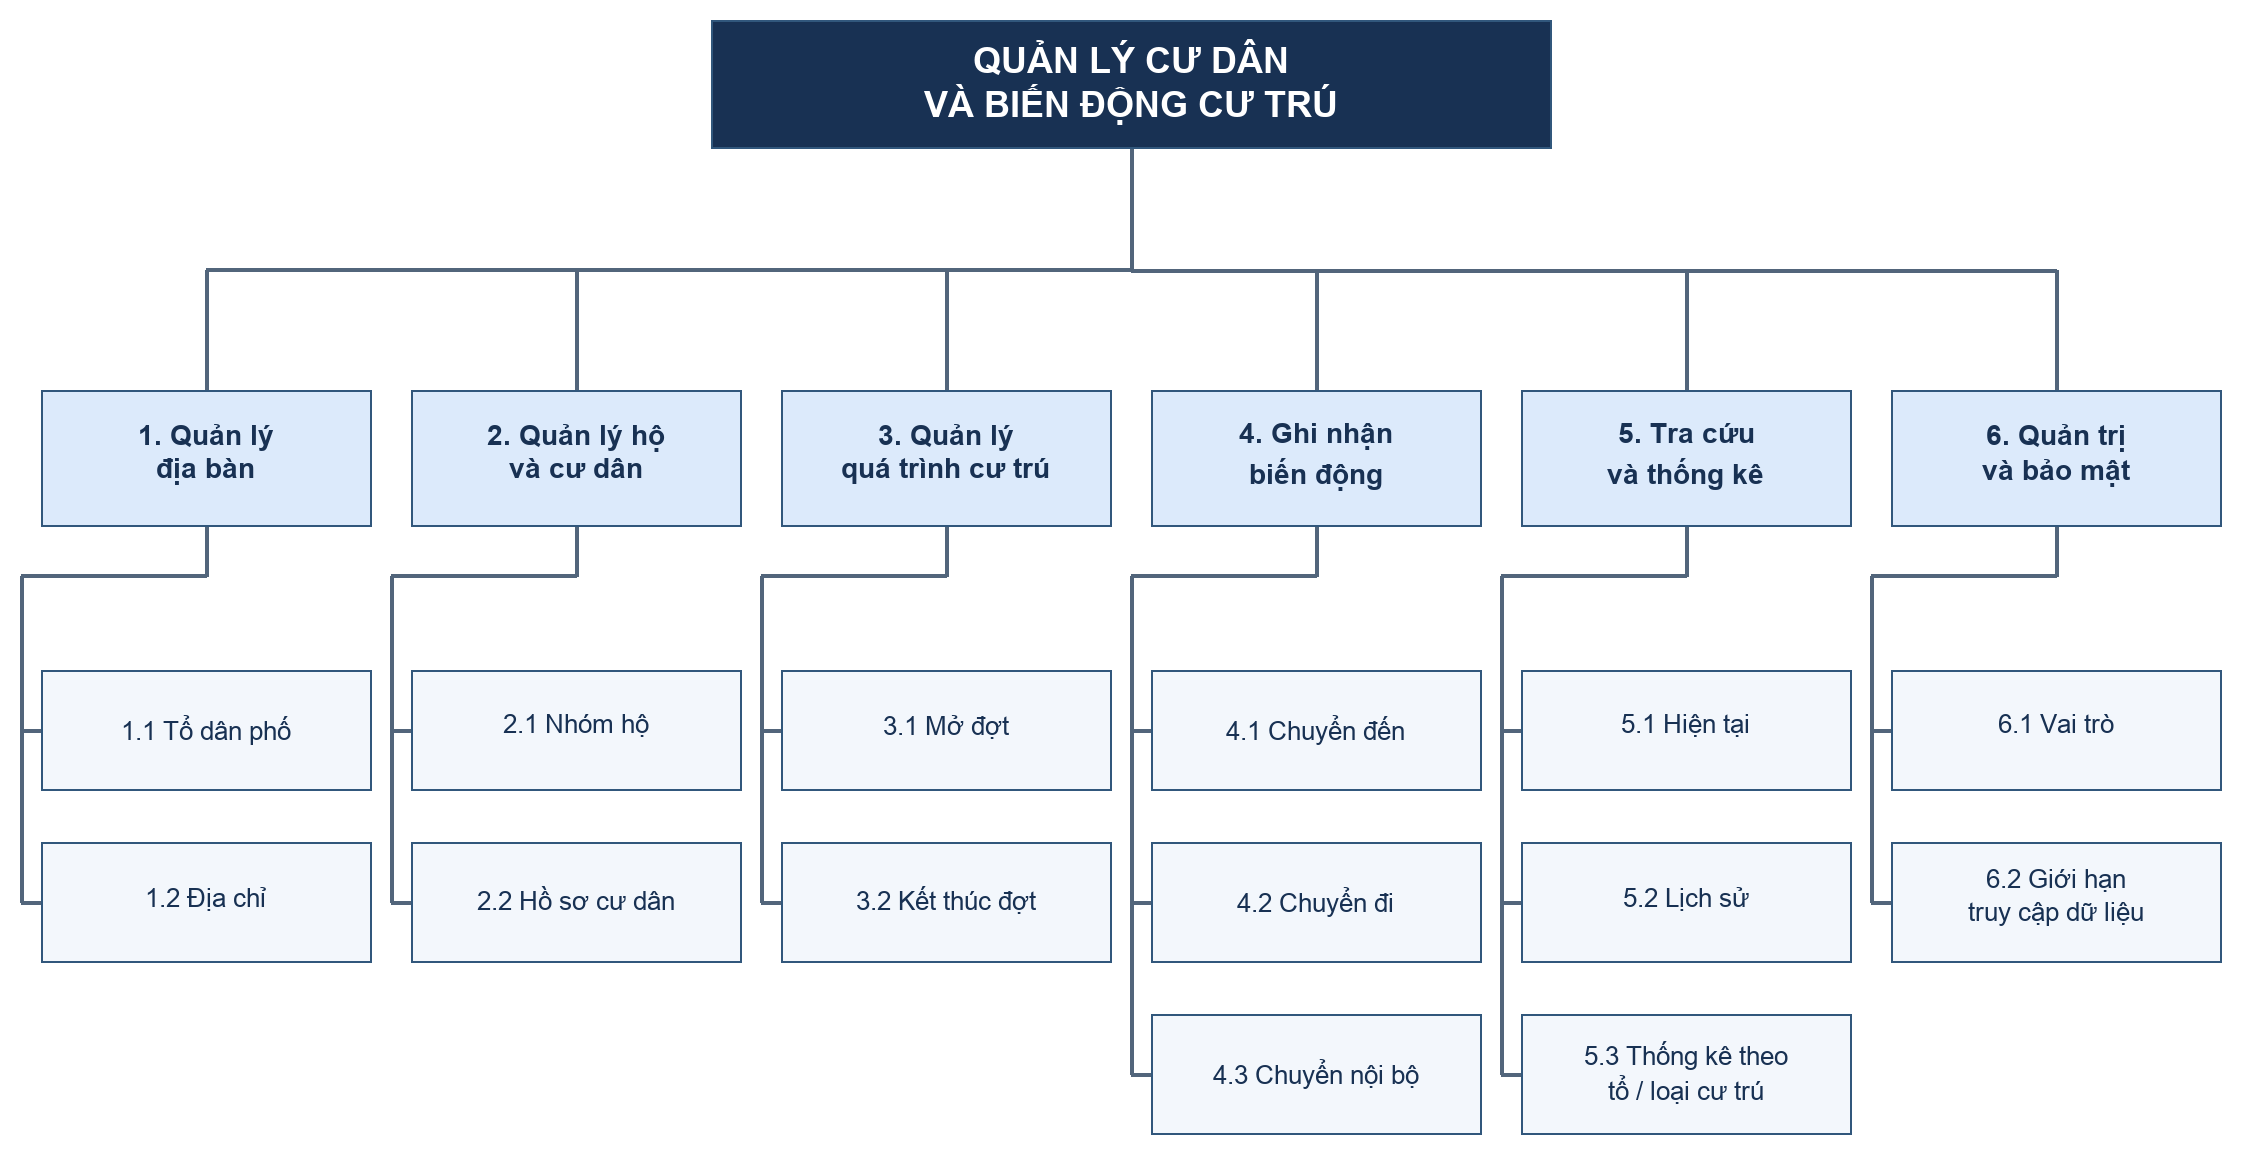
\includegraphics[width=\textwidth]{image/phan_ra_chuc_nang.png}
\caption{Sơ đồ phân rã chức năng của hệ thống quản lý cư dân và biến động cư trú}
\label{fig:bfd}
\end{figure}

Sơ đồ ở Hình \ref{fig:bfd} đọc từ trên xuống: ô trên cùng là toàn bộ hệ thống, hàng thứ hai là sáu nhóm chức năng, các ô dưới mỗi nhóm là 14 chức năng cấp 2 mà người dùng trực tiếp sử dụng.
